\documentclass{bioinfo}
\usepackage{natbib}
\copyrightyear{2009}
\pubyear{2009}

\newcommand{\Rpackage}{`\texttt{#1}'}

\begin{document}
\firstpage{1}

\title[Modular analysis]{Modular analysis of gene expression data with
  GNU R or Matlab}
\author[G\'abor Cs\'ardi \textit{et~al}]{G\'abor Cs\'ardi\,,$^{1,2}$,
  Zolt\'an Kutalik\,$^{1,2}$ and Sven Bergmann\,$^{1,2}$}
\address{$^{1}$Department of Medical Genetics, and 
  $^{2}$Swiss Institute of Bioinformatics,
  University of Lausanne, Rue de Bugnon 27, CH-1005 Lausanne,
  Switzerland.}

\history{Received on XXXXX; revised on XXXXX; accepted on XXXXX}

\editor{Associate Editor: XXXXXXX}

\maketitle

\begin{abstract}

\section{Summary:}
\section{Availability:}
\section{Contact:} \href{Sven.Bergmann@unil.ch}{Sven.Bergmann@unil.ch}
\end{abstract}

\section{Introduction}

% What is biclustering.

Biclustering is the idea of clustering the rows and the columns of a
data matrix, together, usually not independently. In other words, the
goal of a biclustering algorithm is to find blocks in the reordered
data matrix that have, such that the blocks have correlated rows and
columns. It is important to note that these blocks (or biclusters)
have context, i.e. the rows only need to be correlated across the
columns of the block, but not across other columns of the data matrix;
and vice-versa.

When it comes to gene expression data, a bicluster means a subset of
genes ($G$) (or probes, probe sets) and a subset of samples ($S$),
such that genes $G$ are exactly coexpressed across $S$ and samples $S$
have correlated expression profile exactly across $G$.

% What is the ISA.

The Iterative Signature Algorithm (ISA)~\cite{sa,isa,ismod} is a 
powerful biclustering algorithm. It is able to identify biclusters
that overlap and it is resilient to noise.

In this short note, we introduce the \Rpackage{isa2} and
\Rpackage{eisa} GNU R~\cite{R} packages; these implement the ISA
biclustering method, provide a convenient interface to run it using
the BioConductor~\cite{BioC} software package, and also contain
visualization tools.

\section{Methods}

\begin{figure*}
\centering
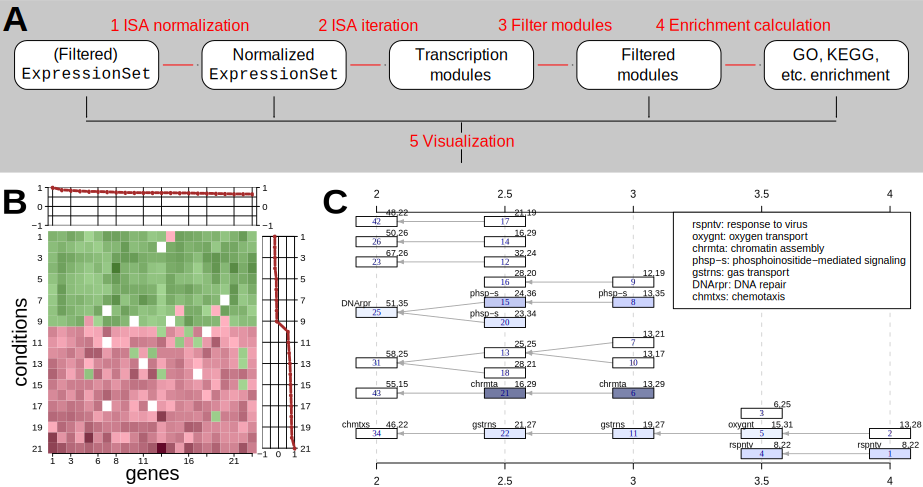
\includegraphics[width=\textwidth]{isa2workflow3}
\caption{}
\label{fig:workflow}
\end{figure*}

% Batch correction

% Normalization. 

% Random and smart seeding. 

% The ISA iteration. 

% Merging the modules.

% The robustness measure and filtering the modules. 

% Module trees.

\section{R Implementation}

Two packages: isa2 does the computation, eisa does everything related
to biology.

\subsection{Work flow}

Two workflows, the simple workflow does everything with default
parameters. In the detailed workflow the user has access to every step
of the analysis.

\subsubsection{The simple work flow}

\subsubsection{The detailed work flow} 

\subsection{Visualization}

Expression plots, GO tree plots, module tree plots, HTML summary
generation. ExpressionView.

\subsection{Connection to other software}

The biclust package.

\section{Matlab implementation}

\section*{Acknowledgement}

\paragraph{Funding\textcolon} 

\paragraph{Conflict of interest\textcolon} None declared.

\bibliographystyle{natbib}
\bibliography{isa}
\nocite{*}

\end{document}
